\documentclass[conference]{IEEEtran}

\usepackage[utf8]{inputenc}
\usepackage[T5]{fontenc}
\usepackage{amsmath,amssymb,amsfonts}
\usepackage{graphicx}
\usepackage{booktabs}
\usepackage{array}
\usepackage{cite}
\usepackage{textcomp}
\usepackage{xcolor}
\usepackage{url}
\usepackage{float}
\usepackage{tikz}
\usetikzlibrary{arrows.meta,positioning,fit,calc,shapes.geometric}

\begin{document}

\title{Bộ Tăng Tốc 2D FFT Cho Xử Lý Ảnh RGB Trên FPGA Zynq-7000}

\author{
    \IEEEauthorblockN{
        Giang Vinh Huy,
        Nguyen Quang Nhon,
        Pham Dinh Phuoc,
        Nguyen Lam Minh Nhat,
        Doan Nhat Hoa
    }
    \IEEEauthorblockA{
        \textit{Department of Computer Engineering}\\
        \textit{Faculty of Electrical and Electronics Engineering}\\
        Ho Chi Minh City University of Technology and Education (HCMUTE)\\
        Ho Chi Minh City, Vietnam
    }
}

\maketitle

\begin{abstract}
    Bài báo này trình bày bộ tăng tốc biến đổi Fourier nhanh hai chiều (2D FFT) cho xử lý ảnh RGB trên nền tảng Zynq-7000/PYNQ-Z1. Hệ thống áp dụng mô hình đồng thiết kế phần cứng/phần mềm, trong đó Processing System chuẩn bị dữ liệu, cấu hình và kiểm tra kết quả, còn Programmable Logic thực hiện khối tính toán FFT. Bộ tăng tốc \textit{fft2d\_fixed\_top} được mô tả bằng C++ trong Vitis HLS, sử dụng thuật toán radix-2, bảng tra hệ số twiddle và biểu diễn số cố định cho ảnh RGB kích thước $64\times64$. IP được tích hợp vào Vivado block design với AXI4-Lite cho điều khiển và AXI master cho truy cập DDR. Thiết kế được kiểm chứng bằng dữ liệu tham chiếu Python/NumPy cùng các báo cáo synthesis, implementation và timing.
\end{abstract}

\begin{IEEEkeywords}
    2D FFT, tăng tốc FPGA, Zynq-7000, Vitis HLS, xử lý ảnh RGB, đồng thiết kế phần cứng/phần mềm.
\end{IEEEkeywords}

\section{Giới Thiệu}
\label{sec:introduction}
Biến đổi Fourier hai chiều là một công cụ quan trọng trong xử lý ảnh số vì cho phép phân tích ảnh trong miền tần số, nơi các đặc trưng như biên, chi tiết nhỏ, nhiễu và kết cấu được thể hiện rõ hơn. Tuy nhiên, phép biến đổi Fourier rời rạc hai chiều (2D DFT) có chi phí tính toán lớn. Thuật toán biến đổi Fourier nhanh (FFT) giảm đáng kể số phép toán bằng cách phân rã phép biến đổi thành các bước nhỏ có cấu trúc lặp lại~\cite{ref:cooley}. Đối với ảnh hai chiều, 2D FFT thường được thực hiện theo phương pháp hàng--cột, tức là FFT một chiều được áp dụng lần lượt trên các hàng và các cột.

Trong các hệ thống nhúng, việc xử lý 2D FFT hoàn toàn bằng CPU có thể gây ra độ trễ cao, đặc biệt với ảnh RGB gồm nhiều kênh dữ liệu. PYNQ-Z1 sử dụng SoC Zynq-7000, kết hợp Processing System (PS) dựa trên ARM và Programmable Logic (PL) trên cùng một chip~\cite{ref:zynq}. Kiến trúc này phù hợp cho đồng thiết kế phần cứng/phần mềm: PS đảm nhiệm chuẩn bị dữ liệu, cấu hình và kiểm tra kết quả, trong khi PL thực hiện phần tính toán FFT có khả năng song song hóa cao.

Dự án này xây dựng bộ tăng tốc 2D FFT cho ảnh RGB kích thước $64\times64$ trên PYNQ-Z1. IP \textit{fft2d\_fixed\_top} được tạo bằng Vitis HLS, tích hợp vào Vivado block design và giao tiếp với PS thông qua AXI4-Lite cho điều khiển và AXI master cho truy cập DDR. Hệ thống tách ảnh thành ba kênh R, G, B, thực hiện 2D FFT riêng cho từng kênh và xuất kết quả phần thực/phần ảo để so sánh với dữ liệu tham chiếu từ Python/NumPy.

Các đóng góp chính của dự án gồm:
\begin{itemize}
    \item Hiện thực bộ tăng tốc 2D FFT cho ảnh RGB $64\times64$ bằng Vitis HLS theo phương pháp hàng--cột.
    \item Tích hợp IP \textit{fft2d\_fixed\_top} vào hệ thống Zynq-7000 với AXI4-Lite điều khiển và AXI master truy cập DDR.
    \item Kiểm chứng thiết kế bằng Python/NumPy và các báo cáo synthesis, implementation, timing.
\end{itemize}

Phần còn lại của bài báo được tổ chức như sau. Mục~\ref{sec:background} trình bày cơ sở lý thuyết, Mục~\ref{sec:methodology} mô tả kiến trúc hệ thống, Mục~\ref{sec:implementation} trình bày quá trình hiện thực, Mục~\ref{sec:results} thảo luận kết quả đánh giá, và Mục~\ref{sec:conclusion} tổng kết các hướng phát triển tiếp theo.

\section{Cơ Sở Lý Thuyết Và Công Trình Liên Quan}
\label{sec:background}
\subsection{Biến Đổi Fourier Nhanh Hai Chiều}
Với một ảnh $f(x,y)$ có kích thước $M\times N$, biến đổi Fourier rời rạc hai chiều (2D DFT) được định nghĩa như sau:
\begin{equation}
    F(u,v)=\sum_{x=0}^{M-1}\sum_{y=0}^{N-1}f(x,y)
    e^{-j2\pi\left(\frac{ux}{M}+\frac{vy}{N}\right)}.
    \label{eq:dft2d}
\end{equation}
2D DFT chuyển ảnh từ miền không gian sang miền tần số, trong đó các hệ số tần số thấp biểu diễn thành phần biến thiên chậm, còn các hệ số tần số cao thể hiện biên, kết cấu và chi tiết nhỏ. Do đó, miền Fourier thường được sử dụng trong lọc ảnh, tăng cường ảnh và phân tích đặc trưng ảnh số~\cite{gonzalez_woods_2018}. Trong đề tài này, ảnh RGB được tách thành ba kênh màu và 2D FFT được áp dụng độc lập trên từng kênh để giữ lại thông tin tần số của từng mặt phẳng màu.

Tính trực tiếp (\ref{eq:dft2d}) đòi hỏi chi phí tính toán lớn vì mỗi hệ số đầu ra phụ thuộc vào toàn bộ mẫu đầu vào. FFT giảm đáng kể độ phức tạp bằng cách phân rã DFT thành các phép toán butterfly nhỏ hơn và khai thác tính đối xứng của nhân Fourier~\cite{cooley_tukey_1965,oppenheim_schafer_2010}. Với dữ liệu hai chiều, phép biến đổi có thể được thực hiện theo phương pháp hàng-cột: tính 1D FFT cho từng hàng, lưu ma trận trung gian, sau đó tính 1D FFT cho từng cột. Cách tổ chức này phù hợp với thiết kế phần cứng vì dùng lặp lại cùng một nhân FFT 64 điểm, có luồng truy cập bộ nhớ rõ ràng và thuận tiện để so sánh kết quả với NumPy \texttt{fft2}.

\subsection{Tăng Tốc FFT Trên FPGA}
FFT phù hợp với FPGA vì thuật toán có cấu trúc đều, gồm các tầng butterfly lặp lại, phép nhân với hệ số twiddle và mẫu truy cập dữ liệu có quy luật. Các đặc điểm này cho phép hiện thực đường dữ liệu chuyên biệt, dùng bộ nhớ trên chip cho dữ liệu trung gian và khai thác song song hóa tốt hơn so với bộ xử lý đa dụng~\cite{parhi_1999}. Tuy nhiên, thiết kế FFT trên FPGA luôn phải cân bằng giữa thông lượng, độ trễ, tài nguyên phần cứng và độ phức tạp điều khiển.

Các kiến trúc FFT có thể ưu tiên pipeline và streaming để tăng thông lượng, hoặc tái sử dụng khối butterfly để giảm tài nguyên. Tài liệu FFT IP của AMD cũng nhấn mạnh các lựa chọn kiến trúc, scaling và xử lý tràn số khi hiện thực FFT fixed-point trên FPGA~\cite{amd_fft_pg109}. Một số nghiên cứu trước đó đã khai thác tái sử dụng tài nguyên và tổ chức bộ nhớ cho các bộ xử lý FFT 1D/2D trên FPGA~\cite{mukherjee_fft_fpga_2015,mukherjee_2dfft_2018}. Trong bài báo này, hướng tiếp cận được chọn là một bộ tăng tốc HLS dễ kiểm chứng, dùng lại nhân radix-2 FFT 64 điểm cho các hàng, cột và ba kênh RGB trên nền tảng Zynq-7000.

\subsection{Số Cố Định Trong HLS}
Số học dấu chấm động thuận tiện khi mô phỏng phần mềm, nhưng thường tiêu tốn nhiều tài nguyên khi tổng hợp lên FPGA. Vì vậy, các thiết kế DSP trên FPGA thường dùng số học dấu chấm cố định để giảm LUT, FF, DSP và giúp dễ đạt timing hơn. Đổi lại, người thiết kế phải lựa chọn hợp lý số bit phần nguyên, số bit phần thập phân, chế độ làm tròn và cơ chế xử lý tràn số.

Vitis HLS cung cấp kiểu \texttt{ap\_fixed}, cho phép mô tả số fixed-point với độ rộng tùy chọn ngay trong C++~\cite{amd_vitis_hls}. Trong FFT, lựa chọn này rất quan trọng vì giá trị trung gian và hệ số DC có thể tăng lớn sau các tầng butterfly; do đó tài liệu FFT IP của AMD xem độ rộng từ, scaling và tràn số là các yếu tố thiết kế cần quan tâm~\cite{amd_fft_pg109}. Trong đề tài này, định dạng \texttt{ap\_fixed<28,20>} được chọn thông qua quá trình quét độ rộng bit và so sánh với kết quả NumPy. Cách chọn này nhằm cân bằng giữa độ chính xác của hệ số FFT và tài nguyên phần cứng trên Zynq-7000.

\subsection{Đồng Thiết Kế Trên Zynq}
Zynq-7000 là nền tảng SoC tích hợp Processing System (PS) dựa trên ARM và Programmable Logic (PL) dựa trên FPGA trong cùng một chip~\cite{xilinx_zynq_trm}. Kiến trúc này phù hợp với các bài toán tăng tốc nhúng, trong đó PS xử lý các tác vụ điều khiển như chuẩn bị dữ liệu, cấu hình tham số và kiểm tra kết quả, còn PL đảm nhiệm các khối tính toán lặp lại và có khả năng song song hóa cao~\cite{rajesh_zynq_codesign_2022}.

Trong đề tài này, bộ tăng tốc 2D FFT được xây dựng như một IP phần cứng được điều khiển bởi phần mềm. PS lưu ảnh RGB trong DDR, cấu hình IP qua AXI4-Lite và cung cấp địa chỉ bộ nhớ đầu vào/đầu ra. PL đọc dữ liệu qua AXI master, thực hiện 2D FFT cho từng kênh màu và ghi kết quả phần thực, phần ảo trở lại DDR. Cách tiếp cận memory-mapped này đơn giản, dễ kiểm chứng và phù hợp với giai đoạn xây dựng phiên bản nền tảng bằng Vitis HLS~\cite{amd_vitis_hls}.

\section{Kiến Trúc Hệ Thống Đề Xuất}
\label{sec:methodology}
\subsection{Tổng Quan Hệ Thống}
Hệ thống đề xuất được tổ chức theo cấu trúc PS/PL của Zynq-7000. PS đảm nhiệm điều khiển ứng dụng, quản lý bộ đệm DDR, bảo trì cache, cấu hình bộ tăng tốc và kiểm tra kết quả. PL chứa IP 2D FFT được sinh từ Vitis HLS. Bộ tăng tốc đọc ảnh RGB đầu vào từ DDR, tính FFT cho từng kênh màu và ghi các ma trận phần thực/phần ảo về DDR. Kiến trúc memory-mapped được chọn cho phiên bản baseline vì dễ kiểm chứng và phù hợp trực tiếp với các giao tiếp AXI4-Lite và AXI master do Vitis HLS sinh ra~\cite{amd_vitis_hls,xilinx_axi_ref}.

\begin{figure*}[t]
    \centering
    \resizebox{0.82\textwidth}{!}{%
        \begin{tikzpicture}[
                font=\scriptsize,
                block/.style={draw, rounded corners, align=center, minimum height=0.75cm, fill=blue!6},
                mem/.style={draw, rounded corners, align=center, minimum height=0.75cm, fill=green!8},
                ip/.style={draw, rounded corners, align=center, minimum height=0.75cm, fill=orange!12},
                bus/.style={-{Latex[length=2.2mm]}, thick},
                dashedbus/.style={-{Latex[length=2.2mm]}, thick, dashed},
                labelbox/.style={fill=white, inner sep=1.5pt, align=center}
            ]
            \node[labelbox] at (3.7,1.75) {\textbf{Zynq-7000 SoC}};
            \node[block, minimum width=4.0cm, minimum height=2.35cm] (ps) at (0,0) {
                \textbf{Processing System (PS)}\\
                ARM Cortex-A9\\[1mm]
                Chuẩn bị bộ đệm\\
                Cấu hình AXI4-Lite\\
                Start/poll và kiểm tra
            };
            \node[block, minimum width=4.6cm, minimum height=2.35cm] (pl) at (7.4,0) {};
            \node[labelbox] at (pl.north) {\textbf{Programmable Logic (PL)}};
            \node[ip, minimum width=3.35cm, minimum height=1.55cm] (fft) at (pl.center) {
                \textbf{IP HLS 2D FFT}\\
                \texttt{fft2d\_fixed\_top}\\[1mm]
                FFT hàng-cột\\
                Twiddle LUT\\
                Datapath fixed-point
            };
            \node[mem, minimum width=10.2cm, minimum height=1.20cm] (ddr) at (3.7,-3.25) {
                \textbf{DDR Memory}\\
                Input RGB buffer \hspace{0.65cm} Output real buffer \hspace{0.65cm} Output imag buffer
            };
            \draw[bus] (ps.east) -- node[labelbox, above] {AXI4-Lite\\điều khiển} (fft.west);
            \draw[bus] (fft.south) -- ++(0,-0.65)
            -- node[labelbox, above] {AXI master đọc/ghi} ++(-2.15,0)
            -- (ddr.north);
            \draw[dashedbus] (ps.south) -- ++(0,-0.70)
            -- node[labelbox, above] {quản lý DDR buffer} ++(-1.60,0)
            -- (ddr.north west);
        \end{tikzpicture}%
    }
    \caption{Kiến trúc tổng quan của bộ tăng tốc 2D FFT trên Zynq.}
    \label{fig:system_overview}
\end{figure*}

Hình~\ref{fig:system_overview} nhấn mạnh sự phân chia giữa điều khiển và tính toán. AXI4-Lite được dùng cho các thanh ghi điều khiển băng thông thấp, còn AXI master memory-mapped được dùng cho đọc/ghi dữ liệu đầu vào và đầu ra. PS chuẩn bị bộ đệm RGB, cấu hình IP HLS, khởi động bộ tăng tốc và kiểm tra kết quả. PL thực hiện các phép FFT hàng-cột lặp lại.

\subsection{Luồng Xử Lý Ảnh RGB}
Ảnh đầu vào được biểu diễn thành ba ma trận $64\times64$ tương ứng với các kênh đỏ, xanh lá và xanh dương. Mỗi kênh được xem như một ảnh vô hướng độc lập. Bộ tăng tốc tính 2D FFT cho từng kênh và tạo hai nhóm đầu ra cho mỗi kênh: hệ số phần thực và hệ số phần ảo.

\begin{figure}[htbp]
    \centering
    \resizebox{\linewidth}{!}{%
        \begin{tikzpicture}[
                font=\scriptsize,
                procstep/.style={draw, rounded corners, align=center, minimum width=2.0cm, minimum height=0.72cm, fill=blue!6},
                fftstep/.style={draw, rounded corners, align=center, minimum width=2.15cm, minimum height=0.72cm, fill=orange!12},
                outstep/.style={draw, rounded corners, align=center, minimum width=2.2cm, minimum height=0.72cm, fill=green!8},
                bus/.style={-{Latex[length=2mm]}, thick}
            ]
            \node[procstep] (input) at (0,0) {Ảnh RGB\\$64\times64$};
            \node[procstep, right=0.65cm of input] (split) {Tách kênh\\R, G, B};
            \node[fftstep, right=0.65cm of split] (row) {FFT 1D\\theo hàng};
            \node[fftstep, right=0.65cm of row] (col) {FFT 1D\\theo cột};
            \node[outstep, right=0.65cm of col] (out) {Đầu ra FFT\\Real/Imag};
            \node[outstep, below=0.65cm of out] (verify) {So sánh NumPy\\MAE/MaxAbs};
            \node[procstep, below=0.65cm of col] (visual) {Hiển thị tùy chọn\\log magnitude};
            \draw[bus] (input) -- (split);
            \draw[bus] (split) -- (row);
            \draw[bus] (row) -- (col);
            \draw[bus] (col) -- (out);
            \draw[bus] (out) -- (verify);
            \draw[bus] (out.south west) -- (visual.north east);
        \end{tikzpicture}%
    }
    \caption{Luồng xử lý ảnh RGB của bộ tăng tốc đề xuất. Hệ số thực và ảo được dùng cho kiểm chứng định lượng, còn phổ log-magnitude chỉ dùng để quan sát trực quan.}
    \label{fig:rgb_pipeline}
\end{figure}

Phổ log-magnitude hữu ích để quan sát trực quan cấu trúc miền tần số, nhưng không được dùng làm tiêu chí đúng sai chính. Kiểm chứng định lượng được thực hiện bằng cách so sánh hệ số thực và ảo thô với kết quả tham chiếu Python NumPy.

\subsection{Phương Pháp FFT Hàng-Cột}
2D FFT được hiện thực bằng phân rã hàng-cột. Với mỗi kênh màu, bộ tăng tốc trước hết thực hiện FFT một chiều trên từng hàng. Kết quả trung gian được lưu trong một ma trận phức nội bộ. Sau đó, bộ tăng tốc thực hiện FFT một chiều trên từng cột của ma trận trung gian và ghi hệ số phần thực/phần ảo cuối cùng vào các bộ đệm đầu ra. Cách phân rã này phù hợp với tính tách biến của 2D DFT và dễ ánh xạ sang C/C++ HLS.

\section{Hiện Thực Phần Cứng/Phần Mềm}
\label{sec:implementation}
\subsection{Kiến Trúc Bộ Tăng Tốc HLS}
Hàm top của HLS được định nghĩa như sau:
\begin{verbatim}
void fft2d_fixed_top(
  data_t input[3][64][64],
  data_t output_real[3][64][64],
  data_t output_imag[3][64][64]);
\end{verbatim}
Khi biên dịch tham chiếu trên desktop, \texttt{data\_t} có thể được định nghĩa là \texttt{double}. Khi tổng hợp bằng Vitis HLS, thiết kế sử dụng \texttt{ap\_fixed<28,20, AP\_RND, AP\_SAT>} làm kiểu số cố định được chọn. Tổng độ rộng 28 bit cung cấp độ chính xác phần thập phân, trong khi 20 bit phần nguyên cung cấp dải biểu diễn đủ lớn cho các giá trị trung gian quan sát được trong các phép thử FFT $64\times64$. Thiết kế dùng kích thước ảnh và số kênh tĩnh, nên cấu trúc vòng lặp và footprint bộ nhớ có tính xác định.

\begin{figure}[htbp]
    \centering
    \resizebox{\linewidth}{!}{%
        \begin{tikzpicture}[
                font=\scriptsize,
                block/.style={draw, rounded corners, align=center, minimum width=2.15cm, minimum height=0.72cm, fill=blue!6},
                fft/.style={draw, rounded corners, align=center, minimum width=2.15cm, minimum height=0.72cm, fill=orange!12},
                mem/.style={draw, rounded corners, align=center, minimum width=2.15cm, minimum height=0.72cm, fill=green!8},
                lut/.style={draw, rounded corners, align=center, minimum width=1.8cm, minimum height=0.65cm, fill=yellow!20},
                bus/.style={-{Latex[length=2mm]}, thick}
            ]
            \node[block] (load) at (0,0) {Nạp ma trận\\một kênh};
            \node[fft, right=0.55cm of load] (rowfft) {FFT radix-2\\theo hàng};
            \node[mem, right=0.55cm of rowfft] (buf) {Bộ đệm\\phức trung gian};
            \node[fft, right=0.55cm of buf] (colfft) {FFT radix-2\\theo cột};
            \node[block, right=0.55cm of colfft] (store) {Ghi đầu ra\\real/imag};
            \node[lut, below=0.65cm of rowfft] (lut1) {Twiddle LUT\\64 điểm};
            \node[lut, below=0.65cm of colfft] (lut2) {Twiddle LUT\\64 điểm};
            \draw[bus] (load) -- (rowfft);
            \draw[bus] (rowfft) -- (buf);
            \draw[bus] (buf) -- (colfft);
            \draw[bus] (colfft) -- (store);
            \draw[bus] (lut1) -- (rowfft);
            \draw[bus] (lut2) -- (colfft);
        \end{tikzpicture}%
    }
    \caption{Datapath nội bộ của bộ tăng tốc 2D FFT hàng-cột. Datapath này được áp dụng độc lập cho các kênh R, G và B.}
    \label{fig:datapath}
\end{figure}

Hình~\ref{fig:datapath} trình bày các khối chính của datapath. Điểm hiện thực quan trọng nhất là thay thế tính toán lượng giác runtime bằng bảng tra twiddle 64 điểm. Cách này tránh việc HLS tổng hợp các phép \texttt{sin} và \texttt{cos} tốn tài nguyên trong datapath, nhờ đó giảm mạnh số DSP, LUT và FF.

\subsection{Phân Chia Phần Cứng/Phần Mềm}
Bảng~\ref{tab:partitioning} tóm tắt cách phân chia phần cứng/phần mềm. Phía phần mềm xử lý các tác vụ điều khiển và kiểm chứng linh hoạt, còn phần cứng thực hiện phần tính toán FFT lặp lại.

\begin{table}[htbp]
    \caption{Phân Chia Phần Cứng/Phần Mềm}
    \centering
    \label{tab:partitioning}
    \begin{tabular}{p{0.22\linewidth}p{0.65\linewidth}}
        \toprule
        \textbf{Thành phần} & \textbf{Nhiệm vụ}                                                                                                                                                                    \\
        \midrule
        PS software         & Chuẩn bị dữ liệu ảnh, quản lý bộ đệm DDR, cấu hình thanh ghi accelerator, flush/invalidate cache, khởi động IP, polling trạng thái hoàn tất, so sánh kết quả với dữ liệu tham chiếu. \\
        PL hardware         & Đọc ma trận đầu vào, tính FFT fixed-point theo hàng và cột cho các kênh R/G/B, áp dụng hệ số twiddle, ghi đầu ra phần thực và phần ảo.                                               \\
        \bottomrule
    \end{tabular}
\end{table}

\subsection{Tổ Chức Bộ Nhớ Và Giao Tiếp AXI}
Kiến trúc baseline sử dụng DDR cho các bộ đệm đầu vào và đầu ra. Bộ đệm đầu vào lưu dữ liệu ảnh RGB, trong khi hai vùng đầu ra lưu hệ số FFT phần thực và phần ảo. Các thanh ghi AXI4-Lite cung cấp thông tin điều khiển và địa chỉ bộ đệm. Các cổng AXI master memory-mapped cho phép accelerator đọc mảng đầu vào và ghi các mảng đầu ra. Cách tổ chức này ưu tiên sự đơn giản trong kiểm chứng; các phiên bản sau có thể bổ sung AXI DMA hoặc AXI Stream để tăng thông lượng.

\subsection{Luồng Kiểm Chứng}
Dự án sử dụng luồng kiểm chứng nhiều tầng như Hình~\ref{fig:verification_flow}. Python NumPy được dùng để sinh kết quả FFT tham chiếu. Hiện thực C++ được kiểm tra trước trên desktop. Phiên bản HLS sau đó được kiểm tra qua C simulation, C synthesis và C/RTL co-simulation. Cuối cùng, nền tảng phần cứng sinh ra được dùng bởi ứng dụng bare-metal Vitis để cấu hình và chạy accelerator trên Zynq.

\begin{figure}[htbp]
    \centering
    \resizebox{\linewidth}{!}{%
        \begin{tikzpicture}[
                font=\scriptsize,
                stage/.style={draw, rounded corners, align=center, minimum width=2.05cm, minimum height=0.70cm, fill=blue!6},
                bus/.style={-{Latex[length=2mm]}, thick}
            ]
            \node[stage] (py) at (0,0) {Python NumPy\\tham chiếu};
            \node[stage, right=0.5cm of py] (cpp) {C++ desktop\\testbench};
            \node[stage, right=0.5cm of cpp] (csim) {HLS\\C simulation};
            \node[stage, below=0.55cm of csim] (syn) {HLS synthesis\\resource/timing};
            \node[stage, left=0.5cm of syn] (cosim) {C/RTL\\co-simulation};
            \node[stage, left=0.5cm of cosim] (board) {Vitis/Zynq\\execution};
            \draw[bus] (py) -- (cpp);
            \draw[bus] (cpp) -- (csim);
            \draw[bus] (csim) -- (syn);
            \draw[bus] (syn) -- (cosim);
            \draw[bus] (cosim) -- (board);
        \end{tikzpicture}%
    }
    \caption{Luồng kiểm chứng nhiều tầng được sử dụng trong dự án.}
    \label{fig:verification_flow}
\end{figure}

\section{Thiết Lập Thực Nghiệm}
Thực nghiệm hướng đến bo mạch PYNQ-Z1 dùng chip Zynq-7000 \texttt{xc7z020clg400-1}. Bộ tăng tốc được tổng hợp bằng AMD Vitis HLS 2025.2 với ràng buộc clock 10 ns. Kích thước đầu vào cố định là ảnh RGB $64\times64$. Bốn mẫu tổng hợp gồm \texttt{square}, \texttt{gradient}, \texttt{checker} và \texttt{circle} được dùng để kiểm chứng định lượng. Kết quả Python NumPy \texttt{fft2} được dùng làm tham chiếu. Sai số được đo trên hệ số FFT thô bằng MAE và MaxAbs cho cả phần thực và phần ảo.

\begin{table}[htbp]
    \caption{Cấu Hình Thực Nghiệm}
    \centering
    \label{tab:experimental_config}
    \begin{tabular}{ll}
        \toprule
        \textbf{Mục}       & \textbf{Cấu hình}                        \\
        \midrule
        Bo mạch            & PYNQ-Z1                                  \\
        FPGA part          & \texttt{xc7z020clg400-1}                 \\
        Toolchain          & AMD Vitis HLS / Vivado / Vitis 2025.2    \\
        Clock mục tiêu     & 10 ns                                    \\
        Clock ước lượng    & 7.300 ns                                 \\
        Kích thước đầu vào & RGB $64\times64$                         \\
        Kiểu dữ liệu chọn  & \texttt{ap\_fixed<28,20>}                \\
        Mẫu kiểm thử       & square, gradient, checker, circle        \\
        Tham chiếu         & Python NumPy \texttt{fft2}               \\
        Thước đo           & Latency, MAE, MaxAbs, BRAM, DSP, FF, LUT \\
        \bottomrule
    \end{tabular}
\end{table}

\section{Kết Quả Và Đánh Giá}
\label{sec:results}
\subsection{Mức Sử Dụng Tài Nguyên}
Tài nguyên phần cứng là thước đo trung tâm của thiết kế vì mục tiêu là triển khai trên FPGA Zynq-7000 có tài nguyên hữu hạn. Bảng~\ref{tab:resource} trình bày ước lượng tài nguyên sau HLS synthesis cho cấu hình được chọn.

\begin{table}[htbp]
    \caption{Mức Sử Dụng Tài Nguyên FPGA}
    \centering
    \label{tab:resource}
    \begin{tabular}{lrrr}
        \toprule
        \textbf{Tài nguyên} & \textbf{Dùng} & \textbf{Tổng} & \textbf{Tỷ lệ} \\
        \midrule
        BRAM\_18K           & 66            & 280           & 23\%           \\
        DSP                 & 8             & 220           & 3\%            \\
        FF                  & 9869          & 106400        & 9\%            \\
        LUT                 & 12375         & 53200         & 23\%           \\
        \bottomrule
    \end{tabular}
\end{table}

DSP chỉ sử dụng 3\%, cho thấy thiết kế còn dư địa để mở rộng song song hoặc bổ sung các khối xử lý ảnh khác. BRAM và LUT là hai nhóm tài nguyên có tỷ lệ sử dụng cao nhất, đạt khoảng 23\%, nhưng vẫn nằm trong khả năng của chip mục tiêu.

\begin{figure}[htbp]
    \centering
    \resizebox{\linewidth}{!}{%
        \begin{tikzpicture}[font=\scriptsize]
            \draw[->] (0,0) -- (7.0,0);
            \draw[->] (0,0) -- (0,3.2) node[above] {Tỷ lệ sử dụng};
            \foreach \y/\lab in {0.5/5\%,1.0/10\%,1.5/15\%,2.0/20\%,2.5/25\%,3.0/30\%} {
                    \draw[gray!35] (0,\y) -- (6.6,\y);
                    \node[left] at (0,\y) {\lab};
                }
            \foreach \x/\name/\h in {0.8/BRAM/2.3,2.2/DSP/0.3,3.6/FF/0.9,5.0/LUT/2.3} {
                    \fill[blue!45] (\x,0) rectangle ++(0.55,\h);
                    \node[below] at (\x+0.28,0) {\name};
                }
            \node[above] at (1.08,2.3) {23\%};
            \node[above] at (2.48,0.3) {3\%};
            \node[above] at (3.88,0.9) {9\%};
            \node[above] at (5.28,2.3) {23\%};
        \end{tikzpicture}%
    }
    \caption{Biểu đồ tỷ lệ sử dụng tài nguyên của thiết kế trên \texttt{xc7z020clg400-1}.}
    \label{fig:resource_utilization}
\end{figure}

\begin{figure*}[t]
    \centering
    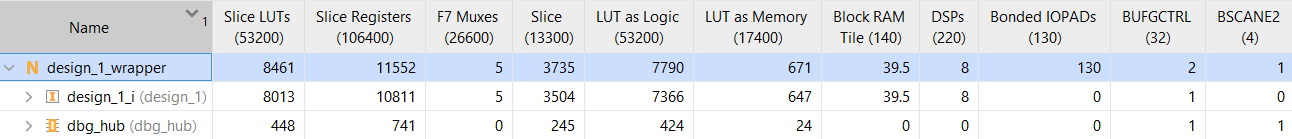
\includegraphics[width=0.96\textwidth]{figures/vivado_implemented_utilization_report.png}
    \caption{Ảnh chụp báo cáo utilization sau implementation trong Vivado cho thiết kế hệ thống. Báo cáo này phản ánh mức sử dụng tài nguyên ở cấp wrapper, bao gồm IP FFT, kết nối AXI, Processing System, khối reset và logic debug.}
    \label{fig:vivado_utilization_report}
\end{figure*}

Ảnh chụp Vivado ở Hình~\ref{fig:vivado_utilization_report} bổ sung góc nhìn sau implementation bên cạnh ước lượng HLS ở Bảng~\ref{tab:resource}. Do phạm vi báo cáo của Vivado là toàn bộ \textit{system wrapper}, các con số không nên được so sánh trực tiếp từng dòng với báo cáo HLS của riêng IP FFT. Tuy vậy, báo cáo này vẫn xác nhận hai điểm quan trọng: thiết kế sau khi tích hợp chỉ sử dụng 8 DSP trên tổng 220 DSP của chip và phần LUT/register vẫn nằm trong giới hạn tài nguyên của \texttt{xc7z020clg400-1}. Điều này giúp củng cố kết luận rằng kiến trúc hiện tại còn đủ dư địa để mở rộng song song hóa hoặc thêm các khối xử lý ảnh phía sau FFT.

\subsection{Ảnh Hưởng Của Tối Ưu Twiddle LUT}
Mức giảm tài nguyên lớn nhất đến từ việc thay thế tính \texttt{sin}/\texttt{cos} runtime bằng bảng tra twiddle 64 điểm. Bảng~\ref{tab:twiddle} so sánh phiên bản dùng lượng giác runtime và phiên bản dùng Twiddle LUT.

\begin{table}[htbp]
    \caption{So Sánh Tối Ưu Twiddle LUT}
    \centering
    \label{tab:twiddle}
    \begin{tabular}{lrrrr}
        \toprule
        \textbf{Phiên bản}                & \textbf{BRAM} & \textbf{DSP} & \textbf{FF} & \textbf{LUT} \\
        \midrule
        Runtime \texttt{sin}/\texttt{cos} & 42            & 186          & 20509       & 29674        \\
        Twiddle LUT                       & 26            & 8            & 10313       & 12126        \\
        \bottomrule
    \end{tabular}
\end{table}

Số DSP giảm từ 186 xuống 8, tương ứng giảm xấp xỉ 95.7\%. FF và LUT cũng giảm hơn một nửa. Kết quả này cho thấy các hàm lượng giác trực tiếp có thể chiếm chi phí lớn trong datapath FFT do HLS sinh ra, và bảng tra là lựa chọn phù hợp cho phép biến đổi có kích thước cố định.

\begin{figure}[htbp]
    \centering
    \resizebox{\linewidth}{!}{%
        \begin{tikzpicture}[font=\scriptsize]
            \draw[->] (0,0) -- (8.2,0);
            \draw[->] (0,0) -- (0,4.2) node[above] {Tài nguyên chuẩn hóa};
            \foreach \y/\lab in {1/25\%,2/50\%,3/75\%,4/100\%} {
                    \draw[gray!35] (0,\y) -- (8.0,\y);
                    \node[left] at (0,\y) {\lab};
                }
            \foreach \x/\name in {0.8/BRAM,2.6/DSP,4.4/FF,6.2/LUT} {
                    \node[below] at (\x+0.28,0) {\name};
                }
            \fill[red!45] (0.55,0) rectangle (0.95,4.00);
            \fill[blue!45] (1.05,0) rectangle (1.45,2.48);
            \fill[red!45] (2.35,0) rectangle (2.75,4.00);
            \fill[blue!45] (2.85,0) rectangle (3.25,0.17);
            \fill[red!45] (4.15,0) rectangle (4.55,4.00);
            \fill[blue!45] (4.65,0) rectangle (5.05,2.01);
            \fill[red!45] (5.95,0) rectangle (6.35,4.00);
            \fill[blue!45] (6.45,0) rectangle (6.85,1.64);
            \node[draw, fill=red!45, minimum width=0.25cm, minimum height=0.15cm] at (6.55,3.80) {};
            \node[right] at (6.75,3.80) {Runtime \texttt{sin}/\texttt{cos}};
            \node[draw, fill=blue!45, minimum width=0.25cm, minimum height=0.15cm] at (6.55,3.45) {};
            \node[right] at (6.75,3.45) {Twiddle LUT};
        \end{tikzpicture}%
    }
    \caption{So sánh tài nguyên giữa phiên bản tính lượng giác runtime và phiên bản dùng bảng tra twiddle.}
    \label{fig:resource_chart}
\end{figure}

\begin{figure*}[t]
    \centering
    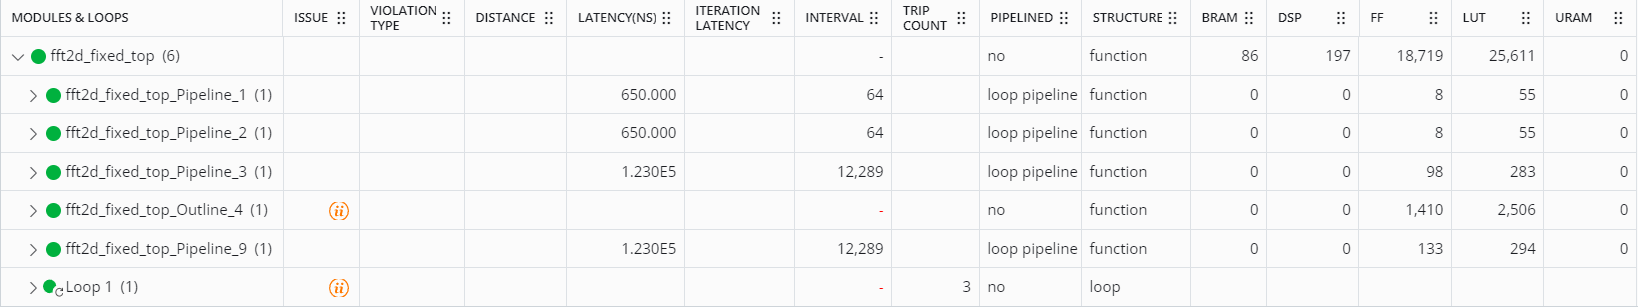
\includegraphics[width=0.96\textwidth]{figures/hls_runtime_trig_resource_report.png}\\[-0.5mm]
    \textbf{(a)} Báo cáo HLS khi hệ số twiddle còn được tính bằng \texttt{sin}/\texttt{cos} runtime.\\[1mm]
    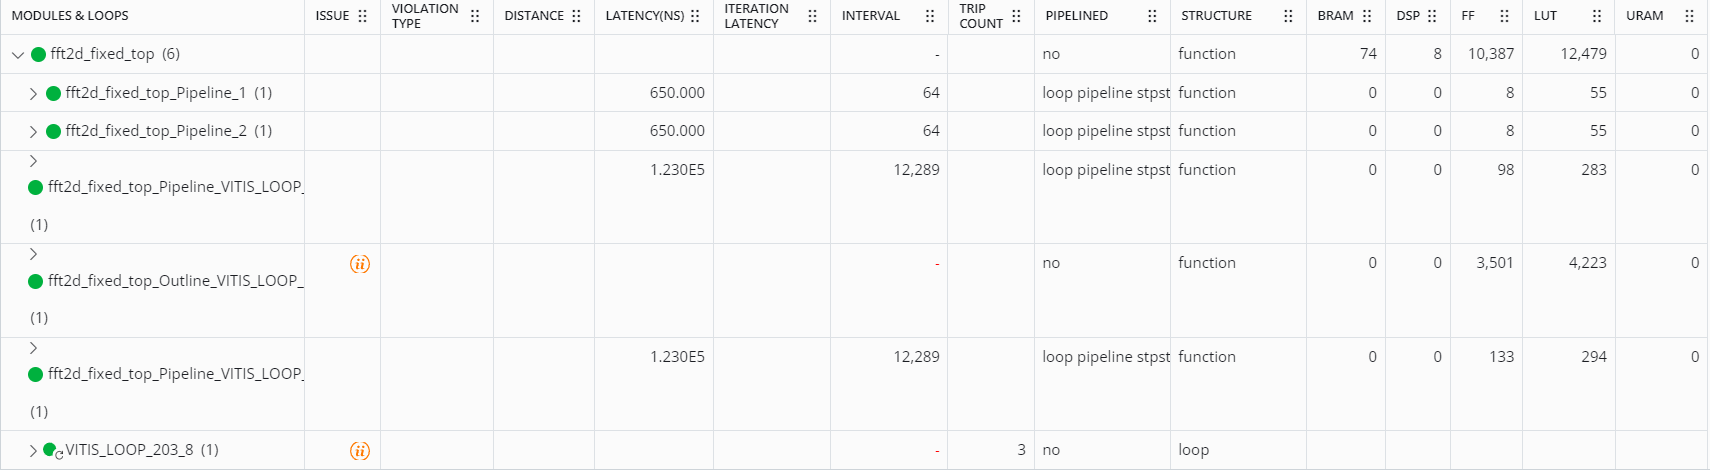
\includegraphics[width=0.96\textwidth]{figures/hls_twiddle_lut_resource_report.png}\\[-0.5mm]
    \textbf{(b)} Báo cáo HLS sau khi thay bằng bảng tra twiddle cố định.
    \caption{Ảnh chụp báo cáo tài nguyên ở mức module/loop của Vitis HLS trong quá trình tối ưu twiddle. Hai ảnh cho thấy xu hướng giảm mạnh DSP và tài nguyên logic khi loại bỏ tính toán lượng giác runtime khỏi datapath FFT.}
    \label{fig:hls_resource_report_screenshots}
\end{figure*}

Hình~\ref{fig:hls_resource_report_screenshots} cho thấy bằng chứng trực tiếp từ giao diện báo cáo HLS trong quá trình tối ưu. Ở phiên bản ban đầu, việc để HLS tổng hợp \texttt{sin}/\texttt{cos} làm cho phần tính twiddle trở thành một thành phần đắt tài nguyên, đặc biệt ở DSP. Sau khi chuyển sang bảng tra cố định, DSP giảm xuống mức rất thấp trong báo cáo HLS, phù hợp với xu hướng đã lượng hóa trong Bảng~\ref{tab:twiddle}. Vì hai ảnh là báo cáo theo cây module/loop trong quá trình phát triển, còn Bảng~\ref{tab:twiddle} là số liệu tổng hợp cuối được chuẩn hóa cho so sánh, bài báo sử dụng bảng làm nguồn số liệu định lượng chính và dùng ảnh chụp như bằng chứng hỗ trợ từ tool.

\subsection{Đánh Giá Bit-Width Fixed-Point}
Nhiều cấu hình fixed-point được đánh giá để tìm điểm cân bằng giữa độ chính xác và tài nguyên FPGA. Bảng~\ref{tab:bitwidth} tóm tắt quá trình sweep bit-width bằng HLS C simulation trên bốn mẫu RGB. Các cấu hình có số bit phần nguyên không đủ đều không vượt qua ngưỡng sai số hiện tại vì FFT $64\times64$ có thể tạo ra giá trị trung gian và đầu ra lớn.

\begin{table*}[t]
    \caption{Sweep Bit-Width Fixed-Point}
    \centering
    \label{tab:bitwidth}
    \begin{tabular}{lrrrl}
        \toprule
        \textbf{Định dạng}        & \textbf{Pass} & \textbf{Worst Real MaxAbs} & \textbf{Worst Imag MaxAbs} & \textbf{Trạng thái} \\
        \midrule
        \texttt{ap\_fixed<32,20>} & 4/4           & 48.1013                    & 34.5814                    & PASS                \\
        \texttt{ap\_fixed<28,20>} & 4/4           & 390.4006                   & 308.7507                   & PASS                \\
        \texttt{ap\_fixed<24,20>} & 0/4           & 4928.0017                  & 3312.7220                  & FAIL                \\
        \texttt{ap\_fixed<22,20>} & 0/4           & 44172.9983                 & 30855.2780                 & FAIL                \\
        \texttt{ap\_fixed<24,16>} & 0/4           & 489472.0039                & 295416.7260                & FAIL                \\
        \texttt{ap\_fixed<24,12>} & 0/4           & 520192.0002                & 326136.7223                & FAIL                \\
        \texttt{ap\_fixed<20,12>} & 0/4           & 520192.0039                & 326136.7260                & FAIL                \\
        \bottomrule
    \end{tabular}
\end{table*}

Cấu hình \texttt{ap\_fixed<28,20>} được chọn vì vượt qua cả bốn mẫu kiểm thử trong khi dùng ít bit hơn \texttt{ap\_fixed<32,20>}. Ước lượng tài nguyên cuối của cấu hình này được trình bày riêng ở Bảng~\ref{tab:resource} dựa trên HLS synthesis của lần co-simulation được báo cáo. Các cấu hình thất bại cho thấy dải biểu diễn phần nguyên quan trọng hơn việc chỉ tăng độ chính xác phần thập phân đối với kích thước FFT baseline này.

\subsection{Độ Chính Xác Và Độ Trễ}
Bảng~\ref{tab:accuracy_latency} trình bày kết quả C/RTL co-simulation được chạy lại cho cấu hình fixed-point được chọn. Tất cả các mẫu đều vượt qua kiểm chứng so với tham chiếu NumPy. Các giá trị MAE và MaxAbs trong bảng được tổng hợp trên cả ba kênh R, G và B; log chi tiết theo từng kênh được lưu trong \texttt{hls/fft2d\_accel/results/cosim\_28\_20\_64}.

\begin{table*}[t]
    \caption{Độ Chính Xác Và Độ Trễ RTL Với \texttt{ap\_fixed<28,20>}}
    \centering
    \label{tab:accuracy_latency}
    \begin{tabular}{lrrrrrl}
        \toprule
        \textbf{Mẫu} & \textbf{Latency} & \textbf{Real MAE} & \textbf{Real MaxAbs} & \textbf{Imag MAE} & \textbf{Imag MaxAbs} & \textbf{Trạng thái} \\
        \midrule
        square       & 1260411          & 1.5991            & 256.3373             & 1.1245            & 91.8750              & PASS                \\
        gradient     & 1260411          & 0.3414            & 93.2577              & 0.5035            & 202.1839             & PASS                \\
        checker      & 1260411          & 1.0716            & 390.4006             & 0.5471            & 308.7507             & PASS                \\
        circle       & 1260411          & 2.9871            & 240.1185             & 2.1791            & 87.1992              & PASS                \\
        \bottomrule
    \end{tabular}
\end{table*}

Độ trễ RTL cố định ở mức 1260411 chu kỳ cho cả bốn mẫu vì kích thước đầu vào và giới hạn vòng lặp là cố định. Ở tần số 100 MHz, độ trễ này tương đương khoảng 12.6 ms cho mỗi frame RGB $64\times64$. Các giá trị MAE nhỏ so với dải động của hệ số FFT thô, cho thấy cấu hình fixed-point được chọn vẫn giữ được hành vi số học mong đợi trên tập kiểm thử hiện tại.

\subsection{Timing Và Công Suất Sau Implementation}
Ngoài tài nguyên logic, timing closure và công suất là hai yếu tố quan trọng để đánh giá khả năng triển khai thực tế của thiết kế~\cite{xilinx_vivado_ug906,xilinx_vivado_ug907}. Hình~\ref{fig:timing_power_reports} trình bày ảnh chụp báo cáo timing và power sau implementation. Báo cáo timing cho thấy tất cả ràng buộc thời gian do người dùng chỉ định đều được đáp ứng, với WNS dương 0.668 ns, WHS dương 0.012 ns và không có endpoint thất bại. Điều này cho thấy thiết kế có thể đóng timing ở cấu hình hiện tại thay vì chỉ dừng ở mức mô phỏng HLS.

\begin{figure*}[t]
    \centering
    \begin{minipage}{0.55\textwidth}
        \centering
        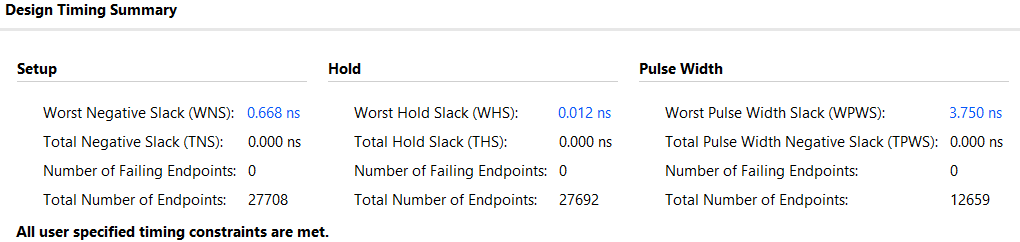
\includegraphics[width=\linewidth]{figures/vivado_timing_summary_report.png}\\[-0.5mm]
        \textbf{(a)} Timing summary sau implementation.
    \end{minipage}
    \hfill
    \begin{minipage}{0.40\textwidth}
        \centering
        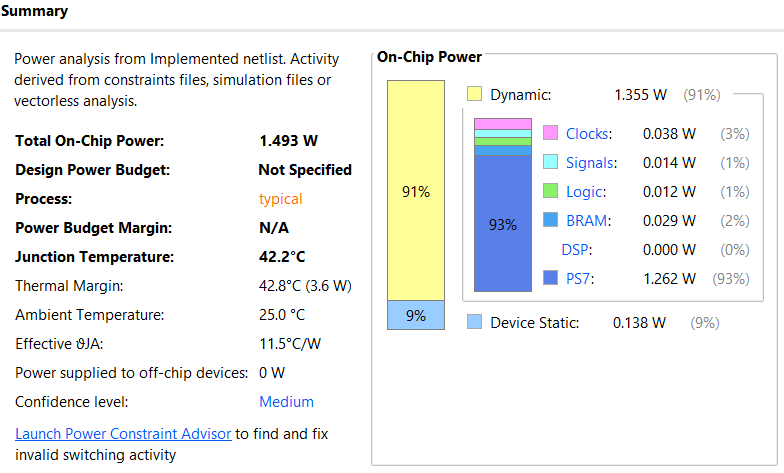
\includegraphics[width=\linewidth]{figures/vivado_power_summary_report.png}\\[-0.5mm]
        \textbf{(b)} Power summary sau implementation.
    \end{minipage}
    \caption{Ảnh chụp báo cáo timing và công suất sau implementation. Timing có slack dương và không có endpoint thất bại; công suất on-chip ước lượng là 1.493 W trong điều kiện activity mặc định/vectorless.}
    \label{fig:timing_power_reports}
\end{figure*}

Về công suất, báo cáo ước lượng tổng công suất on-chip là 1.493 W, trong đó phần động chiếm 1.355 W và phần tĩnh của thiết bị chiếm 0.138 W. Một điểm đáng chú ý là PS7 chiếm tỷ trọng lớn trong công suất động, trong khi logic, BRAM và DSP của phần PL chỉ chiếm tỷ lệ nhỏ. Kết quả này phù hợp với mục tiêu của thiết kế: IP FFT trong PL tiết kiệm DSP và không tạo ra áp lực công suất lớn so với phần hệ thống xung quanh. Tuy nhiên, do báo cáo power được suy ra từ ràng buộc và activity mặc định, kết quả này nên được xem là ước lượng sau implementation; đo công suất thực tế trên bo mạch sẽ là bước cần bổ sung nếu muốn đánh giá năng lượng chính xác hơn.

\subsection{Kiểm Chứng Trực Quan}
\begin{figure}[H]
    \centering
    \scriptsize
    \begin{tabular}{cc}
        
\includegraphics[width=0.23\linewidth]{../../data/demo_fft_tests/input/synthetic_checker_64x64.png}                       &
        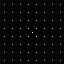
\includegraphics[width=0.23\linewidth]{../../data/demo_fft_tests/python_reference_fft/synthetic_checker_r_fft_python.png}                  \\
        (a) Ảnh đầu vào                                                                                                           & (b) Phổ kênh R \\[0.4mm]
        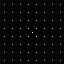
\includegraphics[width=0.23\linewidth]{../../data/demo_fft_tests/python_reference_fft/synthetic_checker_g_fft_python.png} &
        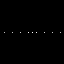
\includegraphics[width=0.23\linewidth]{../../data/demo_fft_tests/python_reference_fft/synthetic_checker_b_fft_python.png}                  \\
        (c) Phổ kênh G                                                                                                            & (d) Phổ kênh B
    \end{tabular}
    \caption{Ảnh RGB đầu vào và phổ FFT log-magnitude dùng cho kiểm chứng trực quan.}
    \label{fig:visual_fft}
\end{figure}

Bên cạnh so sánh định lượng, phổ trực quan giúp xác nhận phép biến đổi tạo ra cấu trúc miền tần số hợp lý. Hình~\ref{fig:visual_fft} minh họa ảnh checker tổng hợp và phổ log-magnitude tham chiếu Python cho các kênh R, G, B sau khi dịch tâm tần số.

Phần hiển thị trực quan không được dùng làm tiêu chí đúng sai chính vì các bước lấy magnitude, lấy log và chuẩn hóa ảnh có thể che khuất sai số ở mức hệ số. Do đó, kết quả định lượng vẫn dựa trên hệ số thực và ảo của FFT.

\section{Thảo Luận}
Kết quả thực nghiệm cho thấy bộ tăng tốc HLS đề xuất là một baseline đúng chức năng và tiết kiệm tài nguyên cho xử lý 2D FFT RGB trên Zynq-7000. Tối ưu Twiddle LUT là cải tiến quan trọng nhất, giảm số DSP khoảng 95.7\% đồng thời giảm đáng kể FF và LUT. Điều này xác nhận rằng các hàm toán học runtime trong HLS cần được xem xét cẩn thận khi nhắm đến FPGA tài nguyên nhỏ.

Kết quả sweep fixed-point cũng cho thấy vai trò quan trọng của số bit phần nguyên. Các định dạng có ít bit phần nguyên thất bại vì FFT có thể sinh ra giá trị trung gian lớn. \texttt{ap\_fixed<28,20>} là lựa chọn cân bằng trong phạm vi thử nghiệm hiện tại: đủ chính xác trên bốn mẫu kiểm thử và tiết kiệm tài nguyên hơn định dạng rộng hơn.

Báo cáo sau implementation bổ sung thêm bằng chứng về tính khả thi của hệ thống khi tích hợp vào Vivado. Thiết kế đóng timing với slack dương, sử dụng 8 DSP ở cấp hệ thống và có công suất on-chip ước lượng 1.493 W. Các số liệu này làm rõ rằng kết quả không chỉ là ước lượng thuật toán ở mức C/HLS, mà đã được kiểm tra qua bước triển khai hệ thống. Dù vậy, cần phân biệt phạm vi báo cáo: HLS phản ánh IP FFT, còn Vivado wrapper bao gồm cả PS, interconnect, reset và debug logic.

Thiết kế hiện tại vẫn có một số giới hạn. Hệ thống chỉ hỗ trợ kích thước $64\times64$, sử dụng datapath memory-mapped baseline và chưa tối ưu cho streaming video liên tục. Tập kiểm thử đủ cho kiểm chứng ban đầu, nhưng cần thêm nhiều ảnh tự nhiên và benchmark lớn hơn trước khi đưa ra kết luận rộng hơn về chất lượng xử lý ảnh hoặc hiệu năng thời gian thực.

\section{Kết Luận Và Hướng Phát Triển}
\label{sec:conclusion}
Bài báo đã trình bày một bộ tăng tốc 2D FFT cho xử lý ảnh RGB trên FPGA Zynq-7000. Thiết kế sử dụng cấu trúc FFT radix-2 hàng-cột, số cố định và bảng tra twiddle 64 điểm. Bộ tăng tốc được kiểm chứng với kết quả Python NumPy thông qua luồng nhiều tầng gồm C simulation và C/RTL co-simulation. Cấu hình được chọn đạt độ trễ RTL 1260411 chu kỳ cho mỗi frame RGB $64\times64$ và sử dụng 66 BRAM\_18K, 8 DSP, 9869 FF và 12375 LUT trên thiết bị mục tiêu.

Trong tương lai, hệ thống có thể được mở rộng theo hướng tăng thông lượng và khả năng mở rộng. Các hướng tiếp theo gồm sử dụng AXI DMA hoặc AXI Stream để truyền dữ liệu, pipeline sâu hơn, xử lý song song các kênh RGB, hỗ trợ kích thước ảnh lớn hơn và tích hợp với camera hoặc pipeline video thời gian thực.

\section*{Lời Cảm Ơn}
Nhóm tác giả xin cảm ơn giảng viên hướng dẫn và các thành viên phòng thí nghiệm đã hỗ trợ trong quá trình thực hiện dự án.

\bibliographystyle{IEEEtran}
\bibliography{zynq_rgb_fft_references}

\end{document}
